% SVN info for this file
\svnidlong
{$HeadURL$}
{$LastChangedDate$}
{$LastChangedRevision$}
{$LastChangedBy$}

\chapter{Conduttori e condensatori}
\labelChapter{conduttori}

\begin{introduction}
	``Mi sento alquanto esausto: mi chiedo che cosa
	deve provare una batteria costretta a riversare elettricità in un non conduttore.''
	\begin{flushright}
		\textscsl{Sherlock Holmes} al dottor John Watson, \emph{L'avventura del detective morente}.
	\end{flushright}
\end{introduction}
\lettrine[findent=1pt, nindent=0pt]{A}{bbiamo} già incontrato, nel \autoref{chap:leggediCoulomb}, una definizione gilbertiana di \textit{conduttore}: ``un materiale che non si elettrizza per strofinio''. È evidente che una definizione così empirica non è particolarmente soddisfacente, anche perché sembra controintuitiva: i metalli sappiamo benissimo che vengono utilizzati negli impianti elettrici, eppure non si elettrizzano?

Questo apparente \textit{paradosso} sta nel concetto stesso di elettrizzazione per strofinio: nei materiali \textit{isolanti}, che si elettrizzano in tale modo, le cariche elettriche rimangono statiche, mentre nei conduttori \textit{sono libere di muoversi}; i fili, piani e sfere cariche che abbiamo studiato in precedenza dovevano necessariamente essere di materiale \textit{isolante}.

In questo Capitolo ci concentreremo invece sui \textbf{conduttori} in condizione di \textit{staticità} - ossia senza movimenti di carica e senza variazioni temporali; vedremo in particolare il \textbf{conduttore cavo} e il suo campo elettrico in diverse situazioni, in quanto ci servirà per studiare i \textbf{condensatori}, dispositivi fisici il cui scopo principale è quello di immagazzinare energia.
\section{Conduttori}
\begin{define}[Conduttore]
	Un \textbf{conduttore}\index{conduttore} è un materiale in cui sono presenti cariche elettriche libere di muoversi.
\end{define}
Per caricare un conduttore possiamo utilizzare diversi metodi, ad esempio con dell'induzione elettrostatica, ma per mantenerlo carico abbiamo bisogno di tenerlo \textit{isolato} da qualunque altro conduttore.

In presenza di un campo elettrico $\vba{E}$, le cariche libere all'interno possono muoversi in modo ordinato e dare vita ad una \textit{corrente elettrica}, ma di questo ci occuperemo nel \autoref{chap:correnteElettrica}. Dato che stiamo studiando i fenomeni elettrostatici, le cariche sono in equilibrio se non abbiamo un \textit{moto di cariche}. Ciò si ha, in termini di condizione media macroscopica, se all'interno del materiale si ha
\begin{equation}
	\vba{E}=0
\end{equation}
Poiché il campo elettrico è nullo, qualunque superficie si consideri \textit{all'interno} del conduttore avrà flusso nullo; per la legge di Gauss, questo significa che \textit{strettamente} all'interno del conduttore \textit{non ci sono cariche}!\\
Con ciò non intendiamo che il corpo \textit{non} è carico - sennò che stiamo a studiarlo? - bensì che non c'è un eccesso di carica di un segno o dell'altro, ma questo eccesso può stare \textit{solo} sulla superficie del conduttore, con distribuzione di carica superficiale
	\begin{equation*}
		\sigma=\pv{q}{\Sigma}
	\end{equation*}
	Per di più, questa distribuzione di carica \textit{non} è generalmente uniforme, bensì si concentrano maggiormente dove il \textbf{raggio di curvatura} è \textit{minore}.
	\begin{center}
		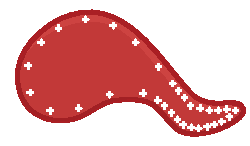
\includegraphics[width=0.35\textwidth]{images/chp4/chp4pipo.pdf}
	\end{center}
\paragraph{I conduttori come superfici equipotenziali}
Un'altra conseguenza fondamentale è che il potenziale deve essere \textit{costante} in ogni punto del conduttore; in particolare ciò è vero sui punti della superficie: la superficie di un conduttore è sempre una \textit{superficie equipotenziale}.\\
In quanto tale, in un punto esterno vicino al conduttore il gradiente del potenziale e quindi il campo elettrico sono ortogonali alla superficie del conduttore, indipendentemente da quale sia la sua forma. Vale pertanto il cosiddetto \textbf{teorema di Coulomb}\index{teorema!di Coulomb}.
	\begin{theoremaqed}[Teorema di Coulomb]
		Il campo elettrico all'esterno di un conduttore con densità superficiale di carica $\sigma$ è
		\begin{equation}
			\tcboxmath[colback=yellowpastellow!30!white,colframe=redsalsa!85!black,drop fuzzy shadow, nobeforeafter, math upper, tcbox raise base, enhanced]{\vba{E}=\frac{\sigma}{\epsilon_0}\vbh{u}_n}\qedhere
		\end{equation}
	\end{theoremaqed}
	Il verso è \textit{uscente} il conduttore se la densità di carica è positiva, \textit{entrante} se è negativa.
\paragraph{Conduttori connessi e potenziale}
Ponendo a contatto due o più conduttori tramite un filo conduttore (trascurabile), si ottiene un \textit{unico corpo conduttore}: all'equilibrio deve valere la condizione $\vba{E}=0$ e $V=\text{const}$, ossia il potenziale - che inizialmente poteva essere differenze su ciascun conduttore - deve diventare uguale su tutti i corpi.	
	\begin{example}
		Consideriamo due sfere di carica $q_i$, densità di carica $\sigma_1$ costante e raggio $R_i$, per $i = 1, 2$. Dato che il campo elettrico esterno è $\vba{E}=\frac{\sigma}{\epsilon_0}\vbh{u}_n$, per continuità del potenziale esse hanno potenziali pari a
		\begin{align*}
			V_1&=\frac{\sigma_1 R_1}{\epsilon_0} & V_2&=\frac{\sigma_2 R_2}{\epsilon_0}
		\end{align*}
		Se le colleghiamo con un filo conduttore trascurabile, all'equilibrio il potenziale diventa unico e pari a $V'_1=V'_2=V$ costante, con $V_i'$ il potenziale su ciascuna sfera dopo averle collegate. Da questa relazione si ottiene come si distribuisce la carica totale
		\begin{equation*}
			q_{tot}=q_1+q_2=q'_1+q'_2
		\end{equation*}
		sulle sfere. Infatti, se $\sigma'_i$ sono le densità di corrente sulle sfere \textit{dopo} averle collegate, si ha
		\begin{gather*}
			V'_1=V'_2\\
			\frac{\sigma'_1R_1}{\Ccancel[red]{\epsilon_0}}=\frac{\sigma'2_2R_2}{\Ccancel[red]{\epsilon_0}}\\
			\frac{q'_1\Ccancel[red]{R_1}}{\Ccancel[red]{4\pi} R_1^{\Ccancel[red]{2}}}=\frac{q'_2\Ccancel[red]{R_2}}{\Ccancel[red]{4\pi} R_2^{\Ccancel[red]{2}}}\\
			\frac{q'_1}{R_1}=\frac{q'_2}{R_2}
		\end{gather*}
		Questa relazione trovata è una riconferma di quanto affermato in precedenza sui raggi di curvatura: più \textit{piccolo} è il \textit{raggio di curvatura}, \textit{maggiore} sarà la \textit{carica} in quei punti (e quindi anche maggiore sarà la densità di carica). Esplicitamente, come si distribuisce la carica tra le due sfere si ricava così:
		\begin{align*}
			q_{tot}&=q'_1+q'_2=q'_1+\frac{R_2}{R_1}q'_1=\frac{R_1+R_2}{R_1}q'_1&\implies q'_1=\frac{R_1}{R_1+R_2}q_{tot}\\
			q_{tot}&=q'_1+q'_2=\frac{R_1}{R_1+R_2}q_{tot}+q'_2 &\implies q'_2=\frac{R_2}{R_1+R_2}q_{tot}
		\end{align*}
	\end{example}
\paragraph{Il campo elettrico indotto}
Per quanto osservato, si può notare come in un conduttore in equilibrio elettrostatico la carica debba avere lo \textit{stesso segno dappertutto} per mantenere $\vba{E}=0$. Questo, tuttavia, non è più vero nel momento in cui il conduttore è \textit{immerso} in un campo elettrico esterno.

Ad esempio, consideriamo due \textit{piastre} cariche di segno opposto in modo che tra di esse si forma un campo elettrico \textit{uniforme} $\vba{E}$, diretto dall'armatura positiva a quella negativa.
Ponendo un conduttore carico in mezzo alle due piastre, le cariche sono soggette ad una forza di Coulomb dovuta alle due piastre e si spostano nel conduttore: le cariche negative si spostano verso la piastra positiva, mentre le positive verso la piastra negativa, come in figura.
\begin{center}
	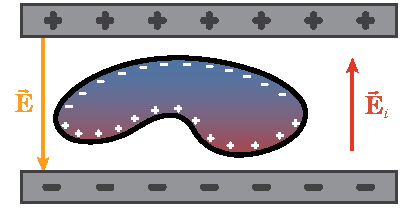
\includegraphics[width=0.6\textwidth]{images/chp4/chp4campoindotto.pdf}
\end{center}
La differenza tra le cariche interne al conduttore crea un \textbf{campo elettrico indotto} $\vba{E}_i$; se lo consideriamo all'equilibrio, esso ha stessa direzione e intensità di $\vba{E}$, ma ha verso opposto in modo da avere all'interno del conduttore la condizione di equilibrio elettrico.
\begin{equation}
	\vba{E}_i=-\vba{E}
\end{equation}
Questo accade in generale anche se il conduttore è immerso in un generico campo elettrico, non necessariamente uniforme o generato da delle armature cariche: per avere l'equilibrio nel conduttore le cariche si devono disporre in modo che la differenza di carica all'interno di esso generi un campo elettrico indotto uguale e opposto a quello del campo elettrico in cui il conduttore è immerso.
\section{Capacità di un conduttore}
Come abbiamo ribadito più volte, parte delle cariche in un conduttore sono libere di muoversi. Se carichiamo un conduttore e poi lo \textit{isoliamo}, possiamo \textit{conservare} della carica elettrica al suo interno - e quindi dell'energia elettrica - che potrà eventualmente essere utilizzata successivamente per altri scopi.

Ci interessa dunque \textit{caratterizzare} i conduttori in base alla loro capacità di caricarsi.
\begin{observe}
	Per studiare un conduttore carico all'equilibrio, dalle osservazioni precedenti ci basta considerarlo come fosse una superficie carica $\Sigma$ con densità di carica $\sigma$. La carica nel conduttore è
	\begin{equation*}
		q=\int_{\Sigma}\sigma\left(x',y',z'\right)d\Sigma
	\end{equation*}
	mentre il potenziale in un qualunque punto del conduttore è
	\begin{equation*}
		V=\frac{1}{4\pi\epsilon_0}\int_{\Sigma}\frac{\sigma(x',y',z')}{\abs{\vba{r}'}}d\Sigma
	\end{equation*}
	dove supponiamo, sempre per le osservazioni precedenti, di considerare l'\textit{origine} del sistema di riferimento scelto all'interno del conduttore e di misurare il potenziale in tale punto - dopotutto, il potenziale è \textit{costante} in tutto il conduttore.
\end{observe}
Ora, osserviamo che se aumentassimo la carica sul conduttore da $q$ a $mq$, si avrebbe un aumento sia della densità di carica di un fattore $m$, sia del potenziale sempre di un fattore $m$. Il loro rapporto, pertanto, rimane costante ed è indipendente da come aumenta la carica e il potenziale: pertanto, esso rappresenta quanto aumenta il potenziale del conduttore all'aumentare della carica. 
\begin{define}[Capacità di un conduttore]
	La \textbf{capacità}\index{capacità} di un conduttore è la misura di quanta carica elettrica bisogna fornire ad un conduttore isolato per aumentare il suo potenziale di un'unità.
	\begin{equation}
		\tcboxmath[colback=yellowpastellow!30!white,colframe=ceruleancrayola!85!black,drop fuzzy shadow, nobeforeafter, math upper, tcbox raise base, enhanced]{C=\frac{q}{V}}
	\end{equation}
\end{define}
Il potenziale in questa definizione è misurato rispetto ad un sistema di riferimento dove lo zero è posto sulla \textit{terra}, considerato un conduttore di dimensioni \textit{infinite} rispetto all'altro e tale per cui se collegassimo il conduttore carico alla terra la carica si disperdesse e il potenziale complessivo è nullo.
\begin{examplewt}[Sfera conduttrice di raggio $R$]
	In una sfera conduttrice di raggio $R$, all'equilibrio la carica è distribuita uniformemente sulla superficie con densità $\sigma$. Si ha
	\begin{align*}
		q&=\int_{\Sigma}\sigma d\Sigma=\sigma\int_{\Sigma}d\Sigma=\sigma A_{sfera}=4\pi R^2 \sigma\\
		V&=\frac{1}{4\pi\epsilon_0}\int_{\Sigma}\frac{\sigma}{\abs{\vba{r}'}}d\Sigma=\frac{1}{4\pi\epsilon_0}\frac{\sigma}{R}\int_{\Sigma}d\Sigma=\frac{1}{\Ccancel[red]{4\pi}\epsilon_0}\frac{\Ccancel[red]{4\pi} R^{\Ccancel[red]{2}} \sigma}{\Ccancel[red]{R}}=\frac{\sigma R}{\epsilon_0}
	\end{align*}
La capacità del conduttore è
\begin{equation}
	C=\frac{q}{V}=4\pi \epsilon_0 R
\end{equation}
Osserviamo che la capacità della sfera non dipende dal materiale, ma solo dal raggio. Questo non è un caso: la capacità è solamente una funzione della \textit{geometria} del conduttore, ma non del materiale con cui è fatto, dalla carica che c'è sopra o dal potenziale in esso (o meglio, differenza di potenziale).
\end{examplewt}
\begin{example}
	Riprendendo il caso delle due sfere conduttrici collegate da un filo trascurabile, come cambia la capacità? La carica complessiva $q_{tot}$ è data dalla somma delle cariche $q_1$ e $q_2$  sulle due sfere, mentre il nuovo potenziale $V$ del sistema è costante e uguale su entrambe le sfere. Segue allora
	\begin{equation}
		C=\frac{q_1+q_2}{V}=\frac{q_1}{V}+\frac{q_2}{V}=4\pi\epsilon_0\left(R_1+R_2\right)=C_1+C_2
	\end{equation} 
	ossia la capacità del sistema di due conduttori collegati da un filo è dato dalla somma delle due capacità dei singoli condensatori.
\end{example}
\paragraph{Unità di misura}
\begin{units}~\\
	\textbf{\textsc{Carica elettrica:}} farad  ($\unit{\farad}$) o coulomb su volt $\left(\unit[per-mode = fraction]{\coulomb\per\volt}\right)$.\\
	\textit{\textbf{Dimensioni:}} $[C]=\dfrac{[q]}{[V]}=\mathsf{M}^{-1}\mathsf{L}^{-2}\mathsf{T}^4\mathsf{I}^2$.
\end{units}
Come per la maggior parte delle unità di misura che si affrontano nell'elettromagnetismo, le capacità utilizzate in ambito pratico sono generalmente di molti ordini di magnitudine minori del farad, cioè siamo praticamente obbligati ad utilizzare sempre dei \textit{sottomultipli} del farad, ad esempio:
\begin{itemize}
	\item \textit{millifarad}: $\SI[per-mode = fraction,exponent-product=\ensuremath{\cdot}]{1}{\milli\farad}=\SI[per-mode = fraction,exponent-product=\ensuremath{\cdot}]{e-3}{\farad}$.
	\item \textit{microfarad}: $\SI[per-mode = fraction,exponent-product=\ensuremath{\cdot}]{1}{\micro\farad}=\SI[per-mode = fraction,exponent-product=\ensuremath{\cdot}]{e-6}{\farad}$.
	\item \textit{nanofarad}: $\SI[per-mode = fraction,exponent-product=\ensuremath{\cdot}]{1}{\nano\farad}=\SI[per-mode = fraction,exponent-product=\ensuremath{\cdot}]{e-9}{\farad}$.
	\item \textit{picofarad}: $\SI[per-mode = fraction,exponent-product=\ensuremath{\cdot}]{1}{\pico\farad}=\SI[per-mode = fraction,exponent-product=\ensuremath{\cdot}]{e-12}{\farad}$.
\end{itemize}
\begin{observe}
		Si osservi che
	\begin{equation*}
		\epsilon_0=\SI[per-mode = fraction,exponent-product=\ensuremath{\cdot}]{8,854e-12}{\square\coulomb\per\newton\square\metre}=\SI[per-mode = fraction,exponent-product=\ensuremath{\cdot}]{8,854e-12}{\farad\per\metre}
	\end{equation*}
\end{observe}
\begin{example}
	Una sfera di rame di raggio
	\begin{itemize}
		\item $R=\SI{0,1}{\metre}$ ha capacità $C=\SI[per-mode = fraction,exponent-product=\ensuremath{\cdot}]{11}{\pico\farad}$.
		\item $R=\SI[exponent-product=\ensuremath{\cdot}]{6,7e6}{\metre}$, cioè una sfera con raggio quello terrestre, ha capacità $C=\SI[per-mode = fraction,exponent-product=\ensuremath{\cdot}]{0,74}{\milli\farad}$.
	\end{itemize}
\end{example}
\section{Conduttore cavo}
Consideriamo un conduttore volumico che non sia pieno, ma che presenta al suo interno una \textit{cavità} senza cariche al suo interno: tale conduttore presenta ora due superfici, una \textit{esterna} e una \textit{interna}. Nel caso del conduttore pieno sappiamo che, all'equilibrio, le cariche si distribuiscono sulla superficie esterna.\\
Sorprendentemente, ciò succede anche nel caso del conduttore cavo: non ci sono cariche nella superficie interna e si distribuiscono \textit{esattamente} come nel caso senza cavità.
\begin{proposition}[Un conduttore cavo ha campo elettrico nullo al suo interno]
	Un conduttore cavo che non presenta cariche all'interno delle cavità si comporta come un conduttore pieno con la stessa geometria. In particolare, le cariche elettriche all'equilibrio si distribuiscono solamente sulla superficie esterna,
\end{proposition}
\begin{demonstration}
	Ricordiamo che, quando consideriamo l'equilibrio elettrostatico, il campo interno al conduttore deve essere nullo.\\
\begin{minipage}{0.35\textwidth}
	\begin{center}
		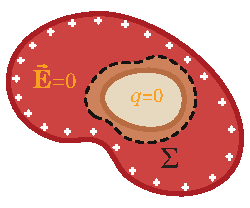
\includegraphics[width=1\textwidth]{images/chp4/chp4condcavodim1.pdf}
	\end{center}
\end{minipage}\hspace{5pt}
\begin{minipage}{0.64\textwidth}
	Prendiamo una superficie $\Sigma$ che circonda completamente la cavità, ma giace interamente all'interno del materiale conduttore.
	Il flusso tramite tale superficie è nullo in quanto il campo elettrico nei punti della superficie è nullo.
	\begin{equation*}
		\Phi_{\Sigma}(\vba{E})=0
	\end{equation*}
\end{minipage}\\
	Applicando la \textit{legge di Gauss}, segue che la carica \textit{complessiva} interna a $\Sigma$ deve essere nulla.
\begin{equation}
	q_{tot,\Sigma\ interna}=0
\end{equation}
Ciò nonostante, questo non preclude ancora la possibilità che ci sia una quantità uguale di cariche positive e negative nella superficie interna del conduttore in modo che	$q_{tot,\Sigma\ interna}$ sia nulla.\\
\begin{minipage}{0.35\textwidth}
	\begin{center}
		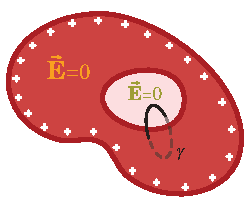
\includegraphics[width=1\textwidth]{images/chp4/chp4condcavodim2.pdf}
	\end{center}
\end{minipage}\hspace{5pt}
\begin{minipage}{0.64\textwidth}
	Per escludere tale possibilità, consideriamo un circuito chiuso $\gamma$ arbitrario che interseca la superficie interna.
	Sappiamo che la \textit{circuitazione} lungo $\gamma$ del campo elettrico è nulla, tuttavia:
	\begin{itemize}
		\item l'integrale di linea lungo la parte di $\gamma$ contenuta nella cavità \textit{non} sarebbe nullo se, per assurdo, ci fossero cariche sulla superficie, dato che ci sarebbe un campo elettrico \textit{non} nullo.
		\item l'integrale di linea lungo la parte di $\gamma$ contenuta nel conduttore sarebbe nullo perché $\vba{E}=0$ dentro il conduttore.
	\end{itemize}
\end{minipage}\\
Pertanto \textit{non} ci possono essere cariche sulla superficie interna e pertanto anche \textit{dentro} la cavità il campo elettrico deve essere nullo.
\end{demonstration}~\\
\begin{minipage}{0.56\textwidth}
Questo è vero anche in presenza di un \textit{campo elettrico esterno} $\vba{E}$. In tal caso, come succede nel conduttore, all'interno della cavità si viene a formare un campo indotto $\vba{E}_i$ dalla separazione delle cariche  che controbilancia quello esterno in modo che il campo complessivo all'interno sia nullo.
\begin{equation*}
	\vba{E}_{tot}=\vba{E}+\vba{E}_i=0
\end{equation*}
\end{minipage}
\begin{minipage}{0.43\textwidth}
\begin{center}
	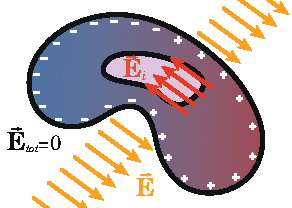
\includegraphics[width=0.8\textwidth]{images/chp4/chp4condcavocampoind.pdf}
\end{center}
\end{minipage}
\subsection{Il conduttore cavo con carica}\label{conduttorecavosfericoconcarica}
\paragraph{Conduttore cavo con carica interna}~\\
\begin{minipage}{0.43\textwidth}
\begin{center}
	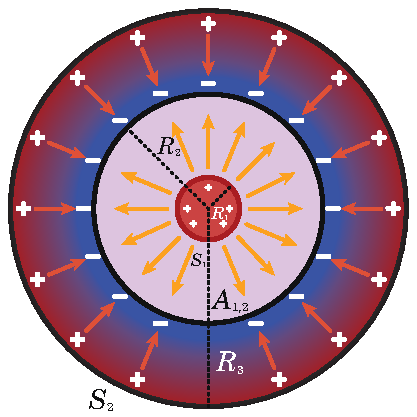
\includegraphics[width=1\textwidth]{images/chp4/chp4sferacavaconsfera.pdf}
\end{center}
\end{minipage}\hspace{10pt}
\begin{minipage}{0.56\textwidth}
Consideriamo, all'equilibrio, una sfera conduttrice cava (inizialmente non carica) di raggio $R_3$ e raggio della cavità $R_2$; al suo interno prendiamo un'ulteriore sfera conduttrice di raggio $R_1<R_2$, e supponiamo che quest'ultima abbia una carica $Q$ positiva.\\
Sappiamo che nella sfera interna il campo elettrico è nullo; la stessa cosa succede sulla \textit{sfera esterna}, ma è meno ovvio.	La sfera carica genera un campo elettrico radiale che, all'esterno di essa, \textit{non} è nullo e attraversa la sfera esterna: le cariche nel conduttore esterno si dispongono come se fosse attraversati da un \textit{campo elettrico esterno}.
\end{minipage}\\
In particolare, le cariche \textit{negative} si posizionano lungo la superficie \textit{interna}, mentre quelle \textit{positive} sono respinte sulla superficie esterna in modo chele cariche sulla superficie interna $q_{int}$ controbilancino quelle sulla superficie esterna $q_{ext}$. Diremo che questo tipo di campo elettrico è un caso di \textbf{induzione totale}.
\begin{define}[Induzione completa]
	Diciamo che si ha \textbf{induzione completa}\index{induzione completa} se le linee di campo elettrico generato da un conduttore terminano completamente in un altro conduttore e, pertanto, il conduttore induce totalmente la sua carica al secondo. 
\end{define}
Ora, consideriamo una superficie ipotetica $\Sigma$ che è contenuta nella sfera esterna e che contiene la cavità. Perché siamo all'equilibrio si ha $\vba{E}=0$, il flusso è
\begin{equation*}
	\Phi_{\Sigma}(\vba{E})=0
\end{equation*}
Ma per la legge di Gauss la carica complessiva è $q_{tot}=0$. Necessariamente, sulla superficie interna deve affacciarsi una carica $q_{int}=-Q$, da cui si ha che $q_{ext}=Q$. Il campo elettrico indotto dovuto dalla disposizione di cariche \textit{controbilancia} quello della sfera interna quindi all'interno del conduttore esterno \textit{non} c'è campo elettrico. Invece, al di fuori del conduttore esterno si verifica nuovamente il campo elettrico dovuto alla sfera carica interna.\\
La situazione è quindi la seguente, al variare della distanza radiale $r$:
\begin{align*}
	E_{r}(r)=\begin{cases}
		0 & r<R_1\\
		\frac{q}{4\pi\epsilon_0r^2} & R_1<r<R_2\\
		0 & R_2<r<R_3\\
		\frac{q}{4\pi\epsilon_0 r^2} & r>R_3
	\end{cases}
	&&
	V(r)=\begin{cases}
		k_1 & r<R_1\\
		\frac{q}{4\pi\epsilon_0r}+k_2 & R_1<r<R_2\\
		k_3 & R_2<r<R_3\\
		\frac{q}{4\pi\epsilon_0r}+k_4 & r>R_3\\
	\end{cases}
\end{align*}
Troviamo le costanti del potenziale imponendo le condizioni al contorno e la continuità:
\begin{align*}
		V(\infty)\displaystyle=\lim_{r\to+\infty}V(r)=0&\implies k_4=0\\
		V_{ext}(R_3)=V_{S_2}(R_3)&\implies k_3=\dfrac{q}{4\pi\epsilon_0R_3}\\
		V_{S_2}(R_2)=V_{A_{1,2}}(R_2)&\implies k_2=\dfrac{q}{4\pi\epsilon_0}\left(\dfrac{1}{R_3}-\dfrac{1}{R_2}\right)\\
		V_{A_{1,2}}(R_1)=V_{S_1}(R_1)&\implies k_1=\frac{q}{4\pi\epsilon_0}\left(\dfrac{1}{R_1}-\dfrac{1}{R_2}+\dfrac{1}{R_3}\right)
\end{align*}
Ricapitolando:
\begin{equation*}
	E_{r}(r)=\begin{cases}
		0 & r<R_1\\
		\frac{q}{4\pi\epsilon_0r} & R_1<r<R_2\\
		0 & R_2<r<R_3\\
		\frac{q}{4\pi\epsilon_0 r} & r>R_3
	\end{cases}
\end{equation*}
\begin{center}
	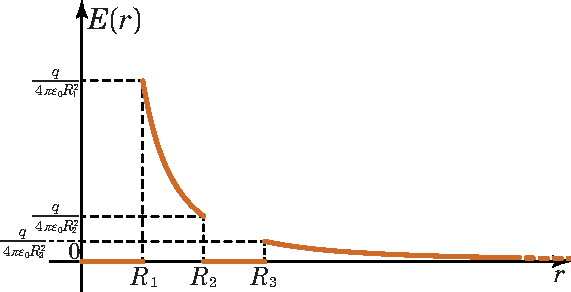
\includegraphics[width=0.75\textwidth]{images/chp4/chp4sferacava2graf1.pdf}
\end{center}
\begin{equation*}
	V(r)=\begin{cases}
		\frac{q}{4\pi\epsilon_0}\left(\frac{1}{R_1}-\frac{1}{R_2}+\frac{1}{R_3}\right) & r<R_1\\
		\frac{q}{4\pi\epsilon_0r}+\frac{q}{4\pi\epsilon_0}\left(\frac{1}{R_3}-\frac{1}{R_2}\right) & R_1<r<R_2\\
		\frac{q}{4\pi\epsilon_0R_3} & R_2<r<R_3\\
		\frac{q}{4\pi\epsilon_0r} & r>R_3\\
	\end{cases}
\end{equation*}
\begin{center}
	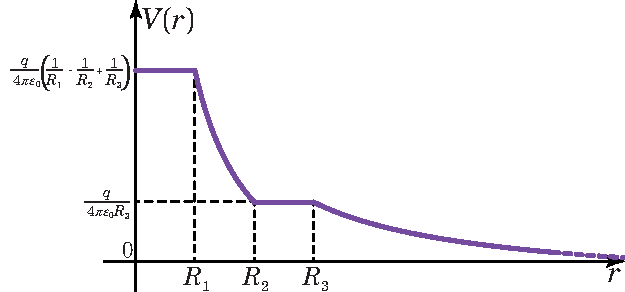
\includegraphics[width=0.75\textwidth]{images/chp4/chp4sferacava2graf2.pdf}
\end{center}
In presenza di un campo elettrico \textit{esterno} si può trovare che, sebbene all'esterno della sfera conduttrice il campo esterno è modificato da quello generato dalla sfera interna, all'interno della cavità è presente \textit{al più} quello dato dalla carica interna.
\paragraph{Conduttore cavo collegato alla carica interna}~\\
\begin{minipage}{0.43\textwidth}
	\begin{center}
		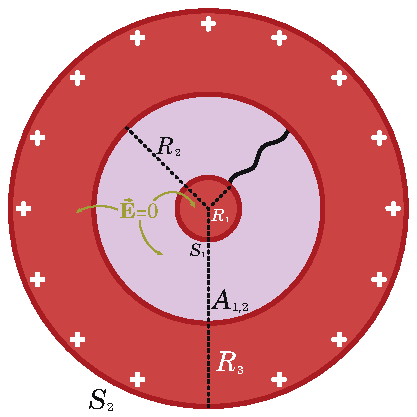
\includegraphics[width=1\textwidth]{images/chp4/chp4sferacavaconsferacollegata.pdf}
	\end{center}
\end{minipage}\hspace{10pt}
\begin{minipage}{0.56\textwidth}
	Colleghiamo le due sfere con un filo conduttore trascurabile. I due conduttori sono ora allo \textit{stesso potenziale} e quindi le cariche su $S_2$s si dispongono sulla superficie della sfera esterna: funzionalmente otteniamo in tutto e per tutto un conduttore cavo \textit{senza alcun oggetto carico nell'ambiente interno}.\\
	Ricapitolando:
	\begin{equation*}
		E_{r}(r)=\begin{cases}
			0 & r<R_3\\
			\frac{q}{4\pi\epsilon_0 r^2} & r>R_3
		\end{cases}
	\end{equation*}
\end{minipage}\\
\begin{center}
	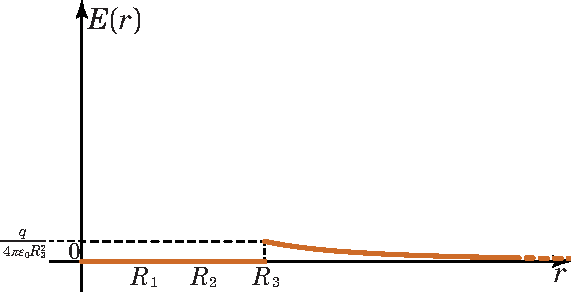
\includegraphics[width=0.65\textwidth]{images/chp4/chp4sferacava3graf1.pdf}
\end{center}
\begin{equation*}
	V(r)=\begin{cases}
		\frac{q}{4\pi\epsilon_0R_3} & r<R_3\\
		\frac{q}{4\pi\epsilon_0r} & r>R_3
	\end{cases}
\end{equation*}
\begin{center}
	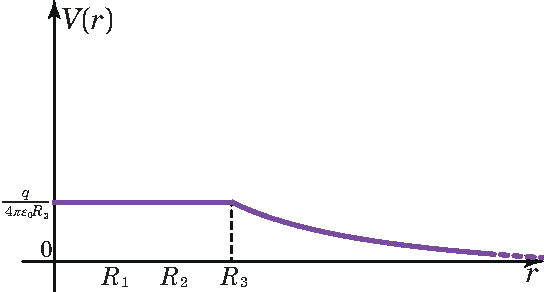
\includegraphics[width=0.65\textwidth]{images/chp4/chp4sferacava3graf2.pdf}
\end{center}
\paragraph{Conduttore cavo collegato alla terra}~\\
\begin{minipage}{0.43\textwidth}
	\begin{center}
		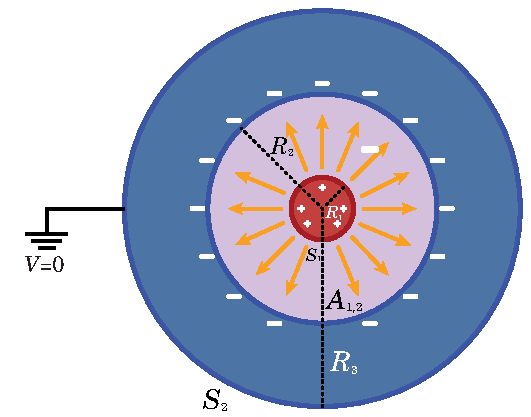
\includegraphics[width=0.9\textwidth]{images/chp4/chp4sferacavaconsferaterra.pdf}
	\end{center}
\end{minipage}\hspace{5pt}
\begin{minipage}{0.56\textwidth}
Supponiamo di riprendere il sistema originale e di collegare il conduttore esterno alla \textit{terra}: in questo modo, le cariche esterne si disperdono nella Terra, dato che la sfera esterna collegata alla terra è come se fosse un unico conduttore di dimensioni \textit{infinite}. Il campo elettrico anche \textit{all'esterno} è \textit{nullo} e, necessariamente, anche il potenziale è \textit{nullo}, dato che il conduttore è allo stesso potenziale della terra, che per convenzione si fissa a $0$.
\end{minipage}\\
Le \textit{uniche} cariche presenti sulla superficie esterna sono le \textit{cariche negative} che si dispongono sulla superficie interna per contrastare il campo elettrico generato dalla carica nella cavità.\\
Ricapitolando:
\begin{equation*}
	E_{r}(r)=\begin{cases}
		0 & r<R_1\\
		\frac{q}{4\pi\epsilon_0 r^2} & R_1<r<R_2\\
		0 & r>R_2
	\end{cases}
\end{equation*}
\begin{center}
	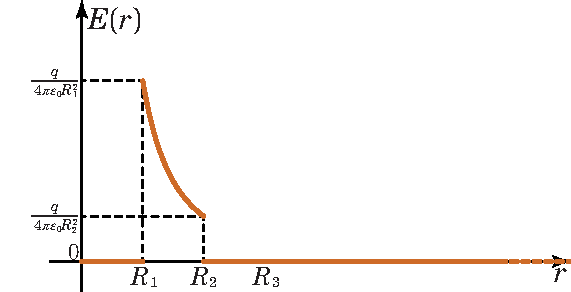
\includegraphics[width=0.75\textwidth]{images/chp4/chp4sferacava4graf1.pdf}
\end{center}
\begin{equation*}
	V(r)=\begin{cases}
		\frac{q}{4\pi\epsilon_0R_1}-\frac{q}{4\pi\epsilon_0R_2} & r<R_1\\
		\frac{q}{4\pi\epsilon_0r}-\frac{q}{4\pi\epsilon_0R_2} & R_1<r<R_2\\
		0 & r>R_2
	\end{cases}
\end{equation*}
\begin{center}
	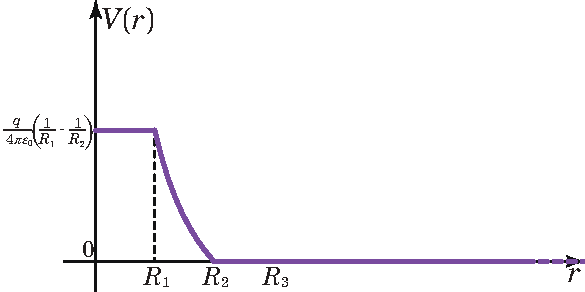
\includegraphics[width=0.75\textwidth]{images/chp4/chp4sferacava4graf2.pdf}
\end{center}
\paragraph{Lo schermo elettrostatico}
Tutti questi esempi ricadono nel fenomeno dello \textbf{schermo elettrostatico}, detto anche \textbf{schermo di Faraday}.
\begin{define}[Schermo elettrostatico o schermo di Faraday]
	Uno \textbf{schermo elettrostatico}\index{schermo elettrostatico}, detto anche \textbf{schermo di Faraday}, è un sistema costituito da un contenitore - non necessariamente continuo - di materiale conduttore in modo da isolare l'ambiente interno da un campo elettrostatico esterno.
\end{define}
\begin{digressionwt}[Gabbia di Faraday]
	Una \textbf{gabbia di Faraday}\index{gabbia di Faraday} è uno schermo di Faraday che presenta delle aperture e, di conseguenza, sono più complesse da analizzare.\\
	Anticipando che i campi elettromagnetici si propagano come onde, uno schermo continuo come il \textit{conduttore cavo} attenua essenzialmente tutte le lunghezze d'onda più corte dello spessore della pelle, i buchi nella gabbia possono permettere alle lunghezze d'onda più corte di attraversarli. Più corta è la lunghezza d'onda, più facilmente passa attraverso una maglia di determinate dimensioni. Così, per lavorare bene con lunghezze d'onda brevi, cioè ad alte frequenze, i fori nella gabbia devono essere \textit{più piccoli} della lunghezza d'onda dell'onda incidente.
\end{digressionwt}
\section{Condensatori}
\begin{define}[Condensatore]
	Un \textbf{condensatore}\index{condensatore} è un sistema di conduttori, i quali sono separati da una differenza di potenziale $\Delta V$ e tra i quali c'è induzione completa.
\end{define}
\begin{notate}
	Spesso abbrevieremo la differenza di potenziale con \ddp
\end{notate}
La maggior parte dei condensatori sono costituite da due o più conduttori elettrici nella forma di piastre metalliche o superfici separate dal vuoto o da un \textit{materiale dielettrico}\footnote{Nel \autoref{chap:dielettrici}, sezione \ref{defdielettrico}, pag. \pageref{defdielettrico}, vedremo la definizione di materiale dielettrico.}, dette \textbf{armature}\index{armatura}.

Dalla legge di Coulomb una carica su un'armatura eserciterà una \textit{forza} sulle cariche dell'altro conduttore, attraendo cariche del segno opposto e respingendo cariche uguali. Per quanto visto con i conduttori cavi, la carica totale $q$ su un'armatura deve essere uguale ma opposte a quella sull'armatura che le sta di fronte, creando un campo elettrico tra i due conduttori.

Lo scopo principale dei condensatori non è solo quello di \textit{deposito} di cariche elettriche nelle armature, ma anche di immagazzinare \textbf{energia elettrica} nel campo elettrico; possiamo crearlo se applichiamo una $\textrm{d.d.p.}$ tra le armature. Per misurare questa proprietà di immagazzinare carica, ci interessa definire, in modo analogo a come abbiamo fatto per i conduttori, una \textbf{capacità} dei condensatori.
\begin{define}[Capacità di un condensatore]
	La \textbf{capacità}\index{capacità} di un condensatore è la misura di quanta carica elettrica bisogna fornire ad un'armatura del condensatore per aumentare di un'unità la \ddp tra le armature.
	\begin{equation}
		\tcboxmath[colback=yellowpastellow!30!white,colframe=ceruleancrayola!85!black,drop fuzzy shadow, nobeforeafter, math upper, tcbox raise base, enhanced]{C=\frac{q}{\Delta V}}
	\end{equation}
\end{define}
Come era per i conduttori, anche la capacità dei condensatori è dipendente esclusivamente dalla \textit{geometria} del conduttore, ma non del materiale con cui è fatto, dalla carica che c'è sopra o dal potenziale in esso (o meglio, differenza di potenziale).
\begin{observe}
	Generalmente, si presuppone di costruire dei condensatori la cui distanza tra le armature sia \textit{molto più piccola} dello spessore delle armature - in modo che sostanzialmente i condensatori considerati siano praticamente uguali anche in termini di dimensioni - e di studiare la differenza di potenziale a debita distanza dal \textit{bordo} in modo da evitare eventuali effetti non graditi.
\end{observe}
\paragraph{Condensatore piano}
Un \textbf{condensatore piano}\index{condensatore!piano} è costituito da due armature piane, distanti $d=x_2-x_1$. Supponiamo che tale distanza sia molto più piccola della larghezza e altezza media delle armature; per dare un confronto dimensionalmente coerente, potremmo dire
\begin{equation}
	d^2\ll \Sigma
\end{equation}
dove $\Sigma$ è l'area della superficie.\\
Il campo elettrico tra due armature piane, lontano dai bordi, si ottiene per il principio di sovrapposizione di due campi $\vba{E}_{+}$ e $\vba{E}_{-}$, generati rispettivamente dalla piastra positiva e dalla piastra negativa. Poiché all'interno delle due piastre tali campi sono concordi e di pari intensità, nota da quanto visto nel  \autoref{chap:FlussoCampoElettrico}, sezione \ref{pianocarico}, pag. \pageref{pianocarico}, si ha dunque
\begin{equation*}
	E(x)=\frac{\sigma}{\epsilon_0}=\frac{q}{\Sigma \epsilon_0}
\end{equation*}
La differenza di potenziale tra le armature è quindi
\begin{equation*}
	\Delta V=V(x_1)-V(x_2)=\left(-\int_{x_0}^{x_1}+\int_{x_0}^{x_2}\right)E(x)dx=\int_{x_1}^{x_2}\frac{q}{\Sigma \epsilon_0}dx=\frac{qd}{\Sigma \epsilon_0}
\end{equation*}
e quindi la capacità del condensatore piano è
\begin{equation}
	\tcboxmath[colback=yellowpastellow!30!white,drop fuzzy shadow, nobeforeafter, math upper, tcbox raise base, enhanced]{C=\frac{\epsilon_0\Sigma}{d}}
\end{equation}
\paragraph{Condensatore cilindrico}
Un \textbf{condensatore cilindrico}\index{condensatore!cilindrico} è costituito da due armature cilindriche: l'armatura interna ha raggio $R_1$, l'esterna ha raggi $R_2$ e $R_3$.
In modo analogo a come abbiamo trovato il campo elettrico di un cilindro uniformemente carico nel \autoref{chap:PotenzialeElettrico}, sezione \ref{supcilindrounifcarica}, pag. \pageref{supcilindrounifcarica}, il campo elettrico nella cavità è
\begin{equation*}
	E(R)=\frac{\sigma R_0}{\epsilon_0 R}=\frac{q}{2\pi\epsilon_0L R},\quad\text{se}\quad R_1<R<R_2
\end{equation*}
e la $\textrm{d.d.p.}$ è
\begin{equation*}
	\Delta V=V(R_1)-V(R_2)=\int_{R_1}^{R_2}E_R(R)dR=\frac{q}{2\pi\epsilon_0L}\log\frac{R_2}{R_1}
\end{equation*}
Se consideriamo la distanza tra le armature \textit{molto più piccola} dei raggi, possiamo considerare le armature come se fossero due cilindri di raggio molto vicino ad $R=R_1$:
\begin{equation*}
	d=R_2-R_1\ll R_1,\ R_2, R_3\implies R_1\sim R_2\sim R_3\sim R
\end{equation*}
Supponiamo, inoltre, di studiare il campo elettrico (e quindi il potenziale) \textit{lontano dai bordi}, onde evitare effetti di bordo non desiderati e difficili da descrivere quantitativamente.
\begin{equation*}
	d\ll L
\end{equation*}
Fissato ciò, si può sviluppare il logaritmo in \textit{serie di Taylor} per ottenere
\begin{equation*}
	\log\frac{R_2}{R_1}=\log\left(1+\frac{R_2-R_1}{R_1}\right)\simeq\frac{d}{R_1}\simeq\frac{d}{R}
\end{equation*}
da cui
\begin{equation*}
	\Delta V=\frac{q}{2\pi\epsilon_0L}\frac{d}{R}
\end{equation*}
e quindi la capacità del condensatore cilindrico è
\begin{equation}
	\tcboxmath[colback=yellowpastellow!30!white,drop fuzzy shadow, nobeforeafter, math upper, tcbox raise base, enhanced]{C=\frac{2\pi\epsilon_0RL}{d}=\frac{\epsilon_0\Sigma}{d}}
\end{equation}
dove $\Sigma=2\pi RL$ è la superficie dell'armatura cilindrica.
\paragraph{Condensatore sferico}
Un \textbf{condensatore sferico}\index{condensatore!sferico} è costituito da due armature sferico: l'armatura interna ha raggio $R_1$, l'esterna ha raggi $R_2$ e $R_3$.
Abbiamo già trovato nella sezione \ref{conduttorecavosfericoconcarica}, \pageref{conduttorecavosfericoconcarica} che il campo elettrico e il potenziale nella cavità sono
\begin{align*}
	E_{r}(r)=\frac{q}{4\pi\epsilon_0r^2}\qquad
	V(r)=\frac{q}{4\pi\epsilon_0r}+\frac{q}{4\pi\epsilon_0}\left(\frac{1}{R_3}-\frac{1}{R_2}\right), \quad\text{se}\quad R_1<r<R_2
\end{align*}
e quindi la \ddp tra le armature è
\begin{equation*}
	\Delta V=V(R_1)-V(R_2)=\int_{R_1}^{R_2}E_r(r)dr=\frac{q}{4\pi\epsilon_0}\left(\frac{1}{R_1}-\frac{1}{R_2}\right)=\frac{q}{4\pi\epsilon_0}\left(\frac{R_2-R_1}{R_1R_2}\right)
\end{equation*}
Se consideriamo la distanza tra le armature \textit{molto più piccola} dei raggi, possiamo considerare le armature come se fossero due sfere di raggio molto vicino ad $R=R_1$:
\begin{equation*}
	d=R_2-R_1\ll R_1,\ R_2, R_3\implies R_1\sim R_2\sim R_3\sim R
\end{equation*}
Fissato ciò, si ha
\begin{equation*}
	\Delta V\simeq\frac{q}{4\pi\epsilon_0}\left(\frac{d}{R^2}\right)
\end{equation*}
e quindi la capacità del condensatore sferico è
\begin{equation}
	\tcboxmath[colback=yellowpastellow!30!white,drop fuzzy shadow, nobeforeafter, math upper, tcbox raise base, enhanced]{C\simeq 4\pi\epsilon_0\left(\frac{R^2}{d}\right)=\frac{\epsilon_0\Sigma}{d}}
\end{equation}
dove $\Sigma=4\pi R^2$ è la superficie dell'armatura sferica.
\section{Il lavoro di carica di un condensatore e l'energia immagazzinata nel condensatore}
Per creare una separazione di carica $q$ nel condensatore, ossia portare la carica $Q$ dalla piastra negativa alla piastra positiva (dal potenziale minore a quello maggiore), una fonte di energia esterna deve compiere un certo \textbf{lavoro} per opporre tale spostamento alla forza del campo elettrico, che la riporterebbe alla piastra originale. L'\textbf{energia elettrica}\index{energia!elettrica} $U$ che viene fornita sotto forma di lavoro $W$ incrementa il potenziale da $0$ fino ad avere una differenza di potenziale $\Delta V$, cioè corrisponde all'energia necessaria per creare partendo da armature scariche il \textit{campo elettrico}. Posto $\Delta V=V(q)-V(0)=V$ e dunque $V=\frac{q}{C}$, si ha
\begin{equation*}
	W=U=\int_{0}^{q}dU=\int_{0}^{q}dV=\int_0^{q}V(Q)dQ=\int_{0}^{q}\frac{Q}{C}dQ=\eval{\frac{1}{2}\frac{Q^2}{C}}_{0}^{q}\frac{q^2}{2C}
\end{equation*}
\begin{equation}
	\tcboxmath[colback=yellowpastellow!30!white,drop fuzzy shadow, nobeforeafter, math upper, tcbox raise base, enhanced]{W=U=\frac{q^2}{2C}=\frac{1}{2}CV^2=\frac{1}{2}qV}
\end{equation}
Questa energia è immagazzinata fondamentalmente nel campo elettrico.
\begin{examplewt}[Condensatore ad armature piane]
	Se consideriamo un condensatore ad armature piane di superficie $\Sigma$ a distanza $d$; il suo campo elettrico tra le armature è
	\begin{equation*}
		E=\frac{\sigma}{\epsilon_0}=\frac{q}{\Sigma \epsilon_0}
	\end{equation*}
	e la sua capacità è
	\begin{equation*}
		C=\frac{\epsilon_0\Sigma}{d}
	\end{equation*}
	L'energia immagazzinata nel condensatore è
	\begin{equation*}
		U=\frac{q^2}{2C}=\frac{E^2\Sigma^{\Ccancel[red]{2}}\epsilon_0^{\Ccancel[red]{2}} d}{2\Ccancel[red]{\epsilon_0}\Ccancel[red]{\Sigma}}=\frac{1}{2}\epsilon_0E^2\Sigma d
	\end{equation*}
\end{examplewt} 
Osserviamo come $\Sigma d$ corrisponde al volume $V$ occupato dal campo elettrico tra le facce del condensatore. Se definiamo la \textbf{densità di energia elettrostatica per unità di volume}\index{densità!di energia!elettraic}
\begin{equation}\label{DensitàEnergiaElettrostatica}
	\tcboxmath[colback=yellowpastellow!30!white,drop fuzzy shadow, nobeforeafter, math upper, tcbox raise base, enhanced]{\mu_{E}=\frac{1}{2}\epsilon_0E^2}
\end{equation}
l'energia immagazzinata nel condensatore è questa densità moltiplicata per il volume $V$ \textit{occupato} dal campo elettrico, confermando che l'energia del condensatore non è conservata nelle piastre, ma nel \textit{campo elettrico}!

\begin{observe}
	Per caricare dei condensatori e immagazzinare nel loro campo elettrico dell'energia possiamo fornire cariche ad una delle armature tramite un collegamento conduttivo esterno, come dei \textit{fili metallici}, e poi scaricare le cariche dall'altra armatura con un altro filo. La quantità di carica che si va a depositare sulle armature è \textit{proporzionale} alla \ddp tra le armature - che possiamo controllare collegando ai capi delle armature una batteria o un generatore con dei fili. Quello che abbiamo descritto non è altro che un semplice \textbf{circuito elettrico}, di cui parleremo meglio nel \autoref{chap:correnteElettrica}
\end{observe}
%Grazie Maccio di esistere - Fra
\section{Energia del campo elettrostatico}
In generale, il campo elettrico immagazzina \textit{sempre} dell'energia nel campo stesso, dato che è l'energia necessaria a separare le cariche richieste per generare il campo elettrico. Tale energia, in un certo volume $V$, è pari a
\begin{equation}
	\tcboxmath[colback=yellowpastellow!30!white,drop fuzzy shadow, nobeforeafter, math upper, tcbox raise base, enhanced]{U=\int_V\mu_EdV=\frac{1}{2}\epsilon_0\int_V\abs{\vba{E}(r)}^2dV}
\end{equation}
dove $\mu_E$ è la densità di energia elettrostatica, definita come nell'equazione \eqref{DensitàEnergiaElettrostatica}.
\section{Pressione elettrostatica}
In un condensatore le piastre sono caricate con segno opposto: questo comporta l'esistenza di una forza che tende a farle \textit{attrarle}. Questa forza è
\begin{equation}
	\vba{F}=-\grad{U}
\end{equation}
dove $U$, nel caso di un condensatore ad armature piane, è
\begin{equation*}
	U=\frac{q^2}{2C}=\frac{q^2d}{2\epsilon_0\Sigma}
\end{equation*}
In modulo, tale forza è
\begin{equation}
	F=\abs{\pdv{U}{d}}=\frac{q^2}{2\epsilon_0\Sigma}
\end{equation}
Si può definire una \textbf{pressione elettrostatica}\index{pressione!elettrostatica} percepita dalle piastre, di intensità
\begin{equation}
	\tcboxmath[colback=yellowpastellow!30!white,drop fuzzy shadow, nobeforeafter, math upper, tcbox raise base, enhanced]{P=\frac{F}{\Sigma}=\frac{q^2}{2\epsilon_0\Sigma^2}=\frac{\sigma^2}{2\epsilon_0}}
\end{equation}